%\documentclass[11pt, english]{book}
\documentclass[]{uiophd}
\usepackage[T1]{fontenc}
\usepackage[utf8x]{inputenc}
%\usepackage[english]{babel}   % S P R A A K
% \usepackage{graphicx}    % postscript graphics
\usepackage{amssymb, amsmath, amsthm} % symboler, osv
\usepackage{mathrsfs}
\usepackage{url}
\usepackage{thmtools}
\usepackage{enumerate}  % lister $  
\usepackage{float}
\usepackage{tikz}
\usepackage{tikz-cd}
\usetikzlibrary{calc}
%\usepackage{tikz-3dplot}
\usepackage{subcaption}
\usepackage[all]{xy}   % for comm.diagram
\usepackage{wrapfig} % for float right
\usepackage{hyperref}
\usepackage{mystyle} % stilfilen      

%\usepackage[a5paper,margin=0.5in]{geometry}


\begin{document}
\title{Smoothing a Calabi-Yau manifold}
\author{Fredrik Meyer}
\maketitle 

\chapter{Preliminary definitions}

We work over $\C$, but some theorems may be stated over a field $k$.

\section{Stanley-Reisner basics}

Given a simplicial complex $\K$, one can associate to it a projective scheme $\PP(\K)$ defined as follows. Let $P$ be the polynomial ring with one variable for each vertex of $\K$. Then the \emph{Stanley-Reisner ideal $I_\K$} corresponding to $\K$ is generated by the monomials corresponding to \emph{non-faces} of $\K$. Then we define the \emph{Stanley-Reisner scheme} to be $\Proj P/I_\K$. 

\begin{example}
Let $\K$ be the square, with vertices $v_0,v_1,v_2,v_3$. Then the Stanley-Reisner ideal is generated by $v_0v_2$ and $v_1v_3$.
\end{example}

Some of the topology of the simplicial complex is encoded in the scheme structure of $\PP(\K)$. In particular, the simplicial (co)homology groups of $\K$ can be computed as the sheaf cohomology of $\PP(\K)$

\begin{lemma}
Let $(K;\C)$ denote the singular cohomology groups of $\K$. Then there are isomorphisms $H^i(K;\C)=H^i(\PP(\K),\OO_{\PP(\K)})$ for all $i$.
\end{lemma}
\begin{proof}
---------to come-----------
\end{proof}

\begin{corr}
We have isomorphisms $H^i(K,\C) \simeq H^{2i}(\PP(\K);\C)$ of singular cohomology groups.
\end{corr}
\begin{proof}
Something about $i$-cells in even dimensions
\end{proof}

\section{Calabi-Yau basics}

\begin{defi}
A \emph{Calabi-Yau variety} is a smooth projective variety satisfying the following two conditions:
\begin{enumerate}
	\item $H^i(X,\OO_X)=0$ for $0 < i < \dim X$.
	\item The canonical sheaf is trivial: $\omega_X \simeq \OO_X$. 
\end{enumerate}
\end{defi}

The classical example of a Calabi-Yau manifold is the quintic threefold in $\PP^5$. Another example is the following:

\begin{example}
Let $X$ be the double cover of $\PP^3$ ramified along a smooth octic. The projection map is affine, so the conditions on $H^i(X,\OO_X)$ are fulfilled. To see that the canonical sheaf is trivial, we use the adjunction formula, which says that $K_X= 2 \restr{K_{\PP^3}}{X} + \deg R$, where $R$ is the ramification divisor. Then, since $\omega_{\PP^3}=\OO_{\PP^3}(-4)$, it follows that $K_X=0$.
\end{example}

If $\K$ is a simplicial sphere, then a smoothing of $\PP(\K)$ will give a Calabi-Yau manifold.


---- ref: bayer-eisenbud graph curves.

The most basic invariants of Calabi-Yau manifolds are their \emph{Hodge numbers $h^{pq}$}. In algebraic geometry these can be defined as the dimensions of the cohomology groups $H^q(X,\Omega^p_X)$. This definition is however not so transparent. On a complex manifold, it is true that $h^{pq}=h^{qp}$, but this is not obvious from our definition. Instead, let us define these groups in complex algebraic geometry terms.

The de Rham complex $(\Omega^\bullet,d)$ refines to a bigraded complex $(\Omega^{\bullet,\bullet},d)$, where a differential form of bidegree $(p,q)$ can be written as 
$$
\omega = \sum {f_{IJ}} dz_{i_1} \wedge \ldots \wedge dz_{i_p} \wedge d\overline{z_1}\ldots \wedge d\overline{z_q}.
$$

The differential $d$ splits as $\partial + \overline \partial$, where $\partial: \Omega^{\bullet,\bullet} \to \Omega^{\bullet+1,\bullet}$, and $\overline \partial: \Omega^{\bullet,\bullet} \to \Omega^{\bullet,\bullet+1}$. The decomposition passes respects cohomology, so we can form the \emph{Dolbeault cohomology groups} $H^{p,q}(X)$. 

With this definition, applying complex conjugation shows that $H^{p,q}=\overline{H^{q,p}}$.

\begin{lemma}
We have natural isomorphisms $H^{p,q}(X) \simeq H^q(X,\Omega_X^p)$. 
\end{lemma}
\begin{proof}
Use that the de Rham complex is flabby
\end{proof}

For more details on this and other details from complex geometry, see  \cite{voisin_complexalg}.

The ``Hodge diamond'' is 
...

\begin{example}
Let $X$ be a smooth quintic in $\PP^4$. We will compute its Hodge numbers. Let us first compute $H^{1,1}(X)$. We have the following exact sequence
$$
0 \to \mathcal I/\mathcal I^2 \to \restr{\Omega_{\PP^4}}{X} \to \Omega_X^1 \to 0
$$
Since $\mathcal I/\mathcal I^2 \simeq \OO_X(-5)$, it follows from the long exact sequence of cohomology that $H^1(X,\Omega^1_X) \simeq H^1(X, \restr{\Omega^1_{PP^4}}{X})$. 
....
\end{example}

\section{Deformation theory}

Deformation theory is the study how varieties (or other algebraic structures like line bundles, vector bundles, ...) vary in families. 

There is a lot of technical machinery available for the deformation theorist, but for us just a few vector spaces will be of importance.

\begin{defi}
Let $X$ be a scheme over $k$. Then a \emph{deformation of $X$ over $S$} is a flat morphism $\mathfrak X \to S$ together with an isomorphism $X \simeq \mathfrak X \times_S 0$ for a closed point $0 \in S$:
$$
\xymatrix{
X \simeq X_0 \ar@{^{(}->}[r] \ar[d] &  \mathfrak X \ar[d] \\
0 \ar[r] & S
}
$$
\end{defi}

Recall that a morphism $f:X \to Y$ is \emph{flat} if the associated morphism $f^{\$}:\OO_Y \to f_\ast \OO_X$ of $\OO_Y$-modules is a flat morphism.

%%% Motivate t1 functors

%% lifting of first order deformations

%% unobstructed problems vs t2 = 0


%%%%%%%%%%%%%%%%%%%%
\chapter{Two topologically distinct smoothings}

Denote by $dP_6$ the del Pezzo surface of degree 6 embedded in $\PP^6$. This can be realized as the blow-up of $\PP^2$ in three points not lying on a line. Let $X$ denote the affine cone over $dP_6$. Then it has long been known that $X$ has two smoothing components, and we show here that they are topologically distinct.

Recall that a \emph{del Pezzo} surface is a surface such that the anti-canonical bundle is ample. The degree is the degree given by the anticanonical embedding. It is a classical result that every del Pezzo surface is obtained either by blowing up $\PP^2$ in $r=0,\ldots,6$ points in suitable positions, or as the $2$-uple embedding of a quadric surface in $\PP^3$. 

\section{Different embeddings of $dP_6$}

We first obtain the equations of $dP_6$ directly from the description of it as blow-up. Let $x_0,x_1,x_2$ be coordinates of $\PP^2$. Recall that the blowup of $\PP^2$ in the point $(1:0:0)$ can be realized as the closed subscheme of $\PP^2 \times \PP^1$ given by the equation $r_0x_1-r_1x_2=0$, where $r_0,r_1$ are coordinates on $\PP^1$. We can repeat this process on the points $(0:1:0)$ and $(0:0:1)$ to obtain similar equations. Collecting these, we see that $dP_6$ is given by the matrix equation
\[
M\vec x = 
\begin{pmatrix}
0 & r_0 & -r_1 \\
s_1 & 0 & -s_0 \\
-t_0 & t_1 & 0
\end{pmatrix}
\begin{pmatrix}
x_0 \\ y_0 \\ z_0
\end{pmatrix}= 0.
\]
in $\PP^2 \times \PP^1 \times \PP^1 \times \PP^1$. Here $r_i,s_i$ and $t_i$ ($i=0,1$) are of course coordinates on $\PP^1$.

We can do more than this however. 

\begin{lemma}
We can also realize $dP_6$ embedded in $\PP^1 \times \PP^1 \times \PP^1$ with equation $r_0s_0t_0=r_1s_1t_1$.
\end{lemma}
\begin{proof}
Note that the matrix cannot have rank $1$ or lower.

Now consider the projection onto the last three factors:
$$
\pi:\PP^2 \times \PP^1 \times \PP^1 \times \PP^1 \to \PP^1 \times \PP^1 \times \PP^1.
$$
Each point $P$ in the product on the right-hand side gives a matrix $M_P$ of rank $2$. Thus there is a line of solutions, which correspond exactly to a point in $\PP^2$.

Hence the restriction of $\pi$ to $dP_6$ is an isomorphism onto the hypersurface given by $\det M=0$ in $\PP^1 \times \PP^1 \times \PP^1$. 
\end{proof}

Another way to realize blow-ups is this: let $\mathfrak d$ be the linear system of quadrics with assigned basepoints $(1:0:0)$, $(0:1:0)$ and $(0:0:1)$ in $\PP^2$. We can choose a basis given by $x_0x_1,x_0x_2$ and $x_1x_2$. This gives a rational map $\PP^2 \rmap \PP^2$. The closure of the graph of this map is a subvariety of $\PP^2 \times \PP^2$ defined by two bilinear equations. Each of the projections correspond to the blowup.

Explicitly, if we let $y_0,y_1,y_2$ be coordinates on the other $\PP^2$, then the equations are $x_1y_0-x_1y_1=x_1y_1-x_2y_2=0$.

We also have a natural embedding in $\PP^6$ as follows. Denote by $E_1, E_2, E_3$ the exceptional divisors on the blowup. Let $L$ be a line in $\PP^2$. Then the divisor $\pi^\ast 3L - E_1-E_2-E_3$ is ample, and gives an embedding in $\PP^6$ (see \cite[Chapter V, Theorem 4.6]{hartshorne}). A basis for the corresponding linear system is given by all monomials in $\Gamma(\PP^2,\OO_{\PP^2}(3))$ except $x^3,y^3$ and $z^3$. 

The equations can be arranged in a particularly symmetric form: let $y,x_1,\ldots,x_1$ be coordinates on $\PP^6$. Then the equations of $dP_6$ are the $2 \times 2$ minors of the matrix
$$
\begin{pmatrix}
x_1 & y & x_6 \\
x_2 & x_3 & y \\
y & x_4 & x_5
\end{pmatrix}.
$$
This gives $9$ equations, which can be compactly written as $x_ix_{i+2}-yx_i=0$ and $x_ix_{i+3}-y^2=0$, for $i=1,\ldots,6$ (where $i$ is taken modulo $6$). Note that the equations have a visible $D_6$-symmetry, where $D_6$ denotes the dihedral group.

\subsection{As a toric variety}

There is a nice combinatorial description of $dP_6$ as a toric variety associated to a polytope. Namely, let $P$ denote the hexagon in \figref{hexagon}. Then the normal fan of this polytope defines a fan in $N_\R$, defining a toric variety.

\begin{figure}
\centering
\begin{subfigure}{.4 \textwidth}
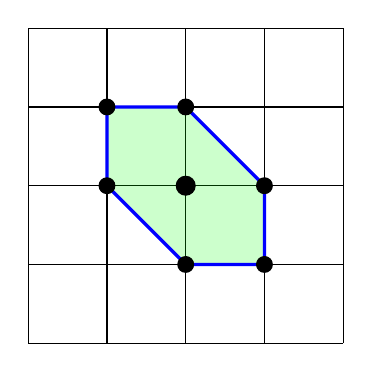
\begin{tikzpicture}
  \draw (0, 0) grid (4, 4);  

\draw [very thick, color=blue, fill=green, fill opacity=0.2]
(2,1) -- (3,1) -- (3,2) -- (2,3) -- (1,3) -- (1,2) -- cycle;

\draw [fill=black]  (2, 1) circle (0.1);
\draw [fill=black]  (3, 1) circle (0.1);
\draw [fill=black]  (3, 2) circle (0.1);
\draw [fill=black]  (2, 3) circle (0.1);
\draw [fill=black]  (1, 3) circle (0.1);
\draw [fill=black]  (1, 2) circle (0.1);
\draw [fill=black]  (2, 2) circle (0.12);
\end{tikzpicture}
\caption{The hexagon.}
\label{fig:hexagon}
\end{subfigure}
\begin{subfigure}{.4 \textwidth}
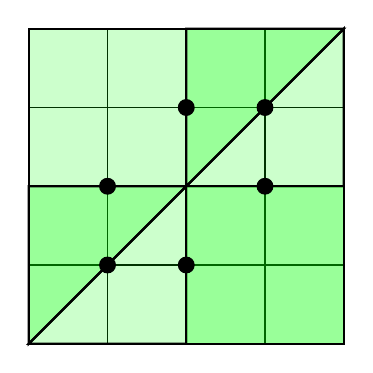
\begin{tikzpicture}
  \draw (0, 0) grid (4, 4);  
%\draw [very thick, fill=green, fill opacity=0.2]
%(1,1) -- (2,1) -- (3,2) -- (3,3) -- (2,3) -- (1,2) -- cycle;
\draw [thick,fill=green, fill opacity=0.2] (2,2) -- (4,2) -- (4,4) -- cycle;
\draw [thick,fill=green, fill opacity=0.4] (2,2) -- (4,4) -- (2,4) -- cycle;
\draw [thick,fill=green, fill opacity=0.2] (2,2) -- (2,4) -- (0,4) -- (0,2) -- cycle;
\draw [thick,fill=green, fill opacity=0.4] (2,2) -- (0,2) -- (0,0) -- cycle;
\draw [thick,fill=green, fill opacity=0.2] (2,2) -- (0,0) -- (2,0) -- cycle;
\draw [thick,fill=green, fill opacity=0.4] (2,2) -- (2,0) -- (4,0) -- (4,2) -- cycle;

\draw [fill=black]  (1, 1) circle (0.1);
\draw [fill=black]  (2, 1) circle (0.1);
\draw [fill=black]  (3, 2) circle (0.1);
\draw [fill=black]  (3, 3) circle (0.1);
\draw [fill=black]  (2, 3) circle (0.1);
\draw [fill=black]  (1, 2) circle (0.1);
%\draw [fill=black]  (2, 2) circle (0.1);
\end{tikzpicture}
\caption{The fan of $dP_6$.}
\label{fig:fandp6}
\end{subfigure}
\caption{Toric description of $dP_6$.}
\end{figure}

The polytope is reflexive, implying that the normal fan of $P$ is the face fan over the same polytope. See \figref{fandp6}. From standard toric geometry, it is clear that $dP_6$ is the blowup of $\PP^2$ in the three torus-fixed points. 

\section{Divisors and topology}

%% Picard group
%% cohomology groups

\section{The affine cone and its two smoothings}

Let $X$ denote the affine cone over $dP_6$. It is an affine variety with an isolated singularity at the origin. One can compute that it has two smoothing components: the union of a plane and a line. They both come from different ways of perturbing the equations of $dP_6$.

\begin{figure}
\centering 
\begin{subfigure}{.4 \textwidth}
  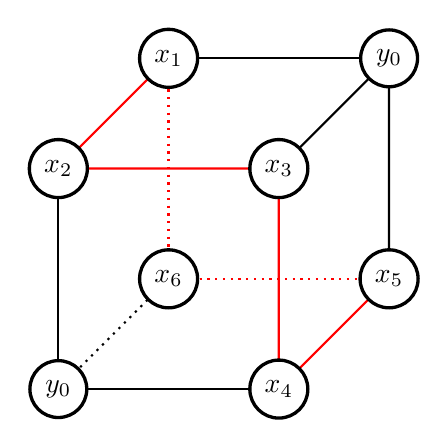
\begin{tikzpicture}[scale=1.4,every node/.style={circle, draw=black, fill=white}, every path/.style={very thick}]
\coordinate (A) at (0,0);
\coordinate (B) at (2,0);
\coordinate (C) at (2,2);	
\coordinate (D) at (0,2);	
\coordinate (E) at (1,1);	
\coordinate (F) at (3,1);	
\coordinate (G) at (3,3);	
\coordinate (H) at (1,3);	
\draw[thick, color=red] (D)  -- (C) -- (B) --(F);  %1
\draw[thick, color=red, dotted] (H) -- (E);
\draw[thick, color=red, dotted] (E) -- (F);
\draw[thick, color=red] (D) -- (H);
\draw[thick] (D) -- (A) -- (B);
\draw[thick] (C) -- (G) -- (F);
\draw[thick] (H) -- (G);
\draw[thick, dotted] (A) -- (E);

\draw (A) node {$y_0$};
\draw (B) node {$x_4$};
\draw (C) node {$x_3$};
\draw (D) node {$x_2$};
\draw (E) node {$x_6$};
\draw (F) node {$x_5$};
\draw (G) node {$y_0$};
\draw (H) node {$x_1$};
\end{tikzpicture}
  \caption{Equations $dP_6$.}
  \label{fig:dp6p1}
 \end{subfigure}
\begin{subfigure}{.4\textwidth}
  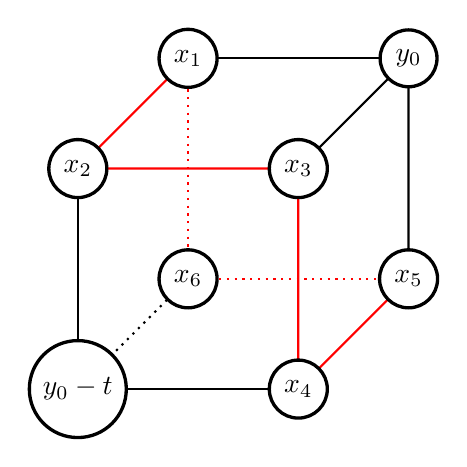
\begin{tikzpicture}[scale=1.4,every node/.style={circle, draw=black, fill=white}, every path/.style={very thick}]
\coordinate (A) at (0,0);
\coordinate (B) at (2,0);
\coordinate (C) at (2,2);	
\coordinate (D) at (0,2);	
\coordinate (E) at (1,1);	
\coordinate (F) at (3,1);	
\coordinate (G) at (3,3);	
\coordinate (H) at (1,3);	

\draw[thick, color=red] (D)  -- (C) -- (B) --(F);  %1
\draw[thick, color=red, dotted] (H) -- (E);
\draw[thick, color=red, dotted] (E) -- (F);
\draw[thick, color=red] (D) -- (H);
\draw[thick] (D) -- (A) -- (B);
\draw[thick] (C) -- (G) -- (F);
\draw[thick] (H) -- (G);
\draw[thick, dotted] (A) -- (E);

\draw (A) node {$y_0-t$};
\draw (B) node {$x_4$};
\draw (C) node {$x_3$};
\draw (D) node {$x_2$};
\draw (E) node {$x_6$};
\draw (F) node {$x_5$};
\draw (G) node {$y_0$};
\draw (H) node {$x_1$};
\end{tikzpicture}
  \caption{Deforming $C(dP_6)$.}
  \label{fig:dp6p12}
  \end{subfigure}
 \caption{Forms of equations.}
\end{figure}

Look at \figref{dp6p1}. One can read off the equations of $dP_6$ by taking minors along ``faces'' and long diagonals of this square. This correspond to a hyperplane cut of $\PP^ 1 \times \PP^1 \times \PP^1$ in the Segre embedding. Then the one-dimensional component of the versal deformation of $X$ is obtained by perturbing one of the $y_0$-corners as in \figref{dp6p12}.

It is clear the corresponding deformation is smooth, since it is a hyperplane cut of cone over $\PP^1 \times \PP^1 \times \PP^1$ outside the origin. Call this smoothing $X_1$.

\begin{lemma}
The smoothing $X_1$ is isomorphic to $\PP^1 \times \PP^1 \times \PP^1 \bs dP_6$.
\end{lemma}
\begin{proof}
Specialize to some $t \neq 0$. Then we can homogenize the equations with respect to $y_1$ to obtain a projective variety in $8$ variables. However, in this form, $y_0-ty_1$ and $y_0$ are linearly independent, hence by a change of variables, we see that this variety is in fact isomorphic to $\PP^1 \times \PP^1 \times \PP^1$ in its Segre embedding.

What we gained by homogenizing is exactly the projective variety given by setting $y_1=0$. But then we get back the equations of $dP_6$ in $\PP^6$.
\end{proof}

The second smoothing is obtained by deforming the equations of $dP_6$ as a subvariety of $\PP^2 \times \PP^2$. Namely, consider the following matrix:

\begin{equation}
\label{eq:def2}
\begin{vmatrix}
x_1 & y_0 & x_6 \\
x_2 & x_3 & y_0-t_1 \\
y_0-t_2 & x_4 & x_5
\end{vmatrix} \leq 1.
\end{equation}


For $t_1=t_2=0$, we get the cone over $dP_6$, while for generic $t_i$, we get a smooth variety. In fact, we can compute that the discrimant locus (the set of points in $\Aa^2_{t_1,t_2}$ with singular fiber) are the $t_1$-axis, the $t_2$-axis and the line $t_1=t_2$. 

Call (any) smooth fiber $X_2$. 

\begin{lemma}
The variety $X_2$ is isomorphic to $(\PP^2 \times \PP^2) \cap H \bs dP_6$, where $H$ is a hyperplane in $\PP^8$.
\end{lemma}
\begin{proof}
The technique is the same as in the previous proof. First homogenize the equations \eqref{eq:def2} with respect to $y_1$. If we let $t_{ij}$ ($i,j=0,1,2$) be coordinates of $\PP^8$, then the homogenized variety is $\PP^2 \times \PP^2 \cap \{h = 0\}$, where $h$ is the hyperplane $(t(t_{32}-t_{11})=s(t_{23}-t_{11}$.

Again, what we gained by homogenizing is given by intersecting with $y_1=0$. But this is exactly $dP_6$ again, in the form $\PP^2 \times \PP^2 \cap \{ t_{23}=t_{32}=0 \}$. 
\end{proof}

We can use what we know about the topology of these spaces to compute homology groups of the two affine smoothings.

\begin{thm}
The two affine smoothings are topologically different. The homology groups are:

\begin{tabular}{ l || c | c | c | c | c | c | c || c }
 Group & 0 & 1 & 2 & 3 & 4 & 5 & 6 & Euler-characteristic \\
\hline
$H^i(X_1,\Z)$ & 1 & 0 & 2 & 1 & 0 & 0 & 0 & 2 \\
$H^i(X_2,\Z)$ & 1 & 0 & 1 & 2 & 0 & 0 & 0  & 0
\end{tabular}
\end{thm}

\begin{proof}
Long exact sequence of a pair + Lefschetz duality 
\end{proof}

\begin{remark}
In fact, the Andreotti-Frankel theorem \cite{andreotti_affinecw} states the following: if $V$ is any smooth affine variety of complex dimension $n$, then it has the homotopy type of a CW complex of dimension $n$.
\end{remark}


%%%%%%%%%%%%%%%%%%%%%%
\chapter{A smooth Calabi-Yau}

Consider the hexagon $E_6$. The join $E_6 \ast E_6$ is a $3$-dimensional sphere, and so a smoothing of the corresponding Stanley-Reisner scheme would correspond to a smooth Calabi-Yau manifold. In this chapter I prove that there does indeed exist a smoothing, and I describe some of its properties.

Description, singularities, etc.


\bibliographystyle{plain}
\bibliography{bibliografi}

\end{document}